
\section{Ergebnisse}

In diesem Kapitel werden die Ergebnisse der einzelnen Zwischenschritte der Methodik nach \autoref{chap:Methodik} dargestellt und kritisch betrachtet.
Hierzu gehören vorerst die Ergebnisse der Clusterung der \gls{MS}-Netzgebiete, die mit \simbev erzeugten Fahrtprofile und Standzeiten von \gls{EPKW} und deren räumlicher Verteilung, sowie die Ergebnisse der Implementierung der verschiedenen Ladestrategien.
Abschließend erfolgt eine detaillierte Betrachtung der Ergebnisse der Ermittlung des Abregelungsbedarfes aufgrund der Integration von \glspl{EPKW} für die untersuchten Netze.


\subsection{Clusterung der MS-Netzgebiete}

% TODO: Auswertungen von Birgit übernehmen. Balkendiagramm

Die vollständige Untersuchung der mit Hilfe des Software Tools \dingo synthetisierten \gls{MS}-Netzgebiete, würde aufgrund ihrer großen Anzahl zu inakzeptabel hohen Rechenzeiten führen.
Im Rahmen dieser Masterarbeit wurden sechs Referenznetzgebiete ausgewählt, welche \num{1842} der \num{3591} {\color{red} TODO 3354?} \gls{MS}-Netze repräsentieren.
Das Clustering erfolgte innerhalb \cite{Schachler} durch den während des \openego Projektes entwickelten k-means-Clusteralgorithmus nach \autoref{chap:dingo_theo}.\medskip

Um mit dieser Arbeit eine Ergänzung zu \cite{Schachler} zu liefern, wurde das Clustering übernommen.
Von den \num{15} identifizierten repräsentativen Netzgebieten wurde eine Teilmenge für die Untersuchung ausgewählt.
So wurden jeweils zwei Netzgebiete der Kategorien Wind-, \gls{PV}- und Last-dominiert ausgewählt, die möglichst viele Netzgebiete repräsentieren, damit die Effekte der Netzintegration der Elektromobilität auf möglichst unterschiedliche Netze gezeigt werden kann.
Insgesamt wurden somit \num{6} Netzgebiete untersucht, die stellvertretend für \num{1842} der \num{3591} Mittelspannungsnetze stehen.
In \autoref{tab:grid_IDs} finden sich die \glspl{ID} der untersuchten Mittelspannungsnetze und die Anzahl an repräsentierten Netzgebieten.

{
\renewcommand{\arraystretch}{1.2}% grßerer Zeilenabstand
\sisetup{range-phrase=~{--}~}% Gedankenstrich statt "bis" bei SIrange
\begin{table}[H]
	\begin{center}
		\caption{Anzahl der repräsentierten Netzgebiete und Kategorie der untersuchte Mittelspannungsnetze}
		\begin{tabu} to \textwidth {X[1] X[1] X[1, r] }
			\hline
			Netz ID    & Kategorie      & Anzahl repräsentierter Netze \\ \hline
			\num{176}  & PV-dominiert   & \num{413}                    \\
			\num{177}  & Last-dominiert & \num{666}                    \\
			\num{1056} & PV-dominiert   & \num{197}                    \\
			\num{1690} & Wind-dominiert & \num{141}                    \\
			\num{1811} & Wind-dominiert & \num{78}                     \\
			\num{2534} & Last-dominiert & \num{347}                    \\ \hline
		\end{tabu}
		\label{tab:grid_IDs}
	\end{center}
	\vspace{-3mm}%Put here to reduce too much white space after your table
\end{table}
}


In {\color{red} TODO} findet sich eine Darstellung der wichtigsten Charakteristika der untersuchten Netzgebiete.
Hierzu zählen die installierten \gls{PV}- und Wind-Kapazitäten, sowie die Spitzenlast der \glspl{EPKW} und \glspl{WP}.
Weiterhin findet sich in \autoref{fig:map_representatives} eine Karte der repräsentierten Netzgebiete eingeteilt in die Kategorien Wind-, \gls{PV}- und Last-dominiert.

{\color{red} TODO: BAR Plot grids}

\begin{figure}
    \centering
    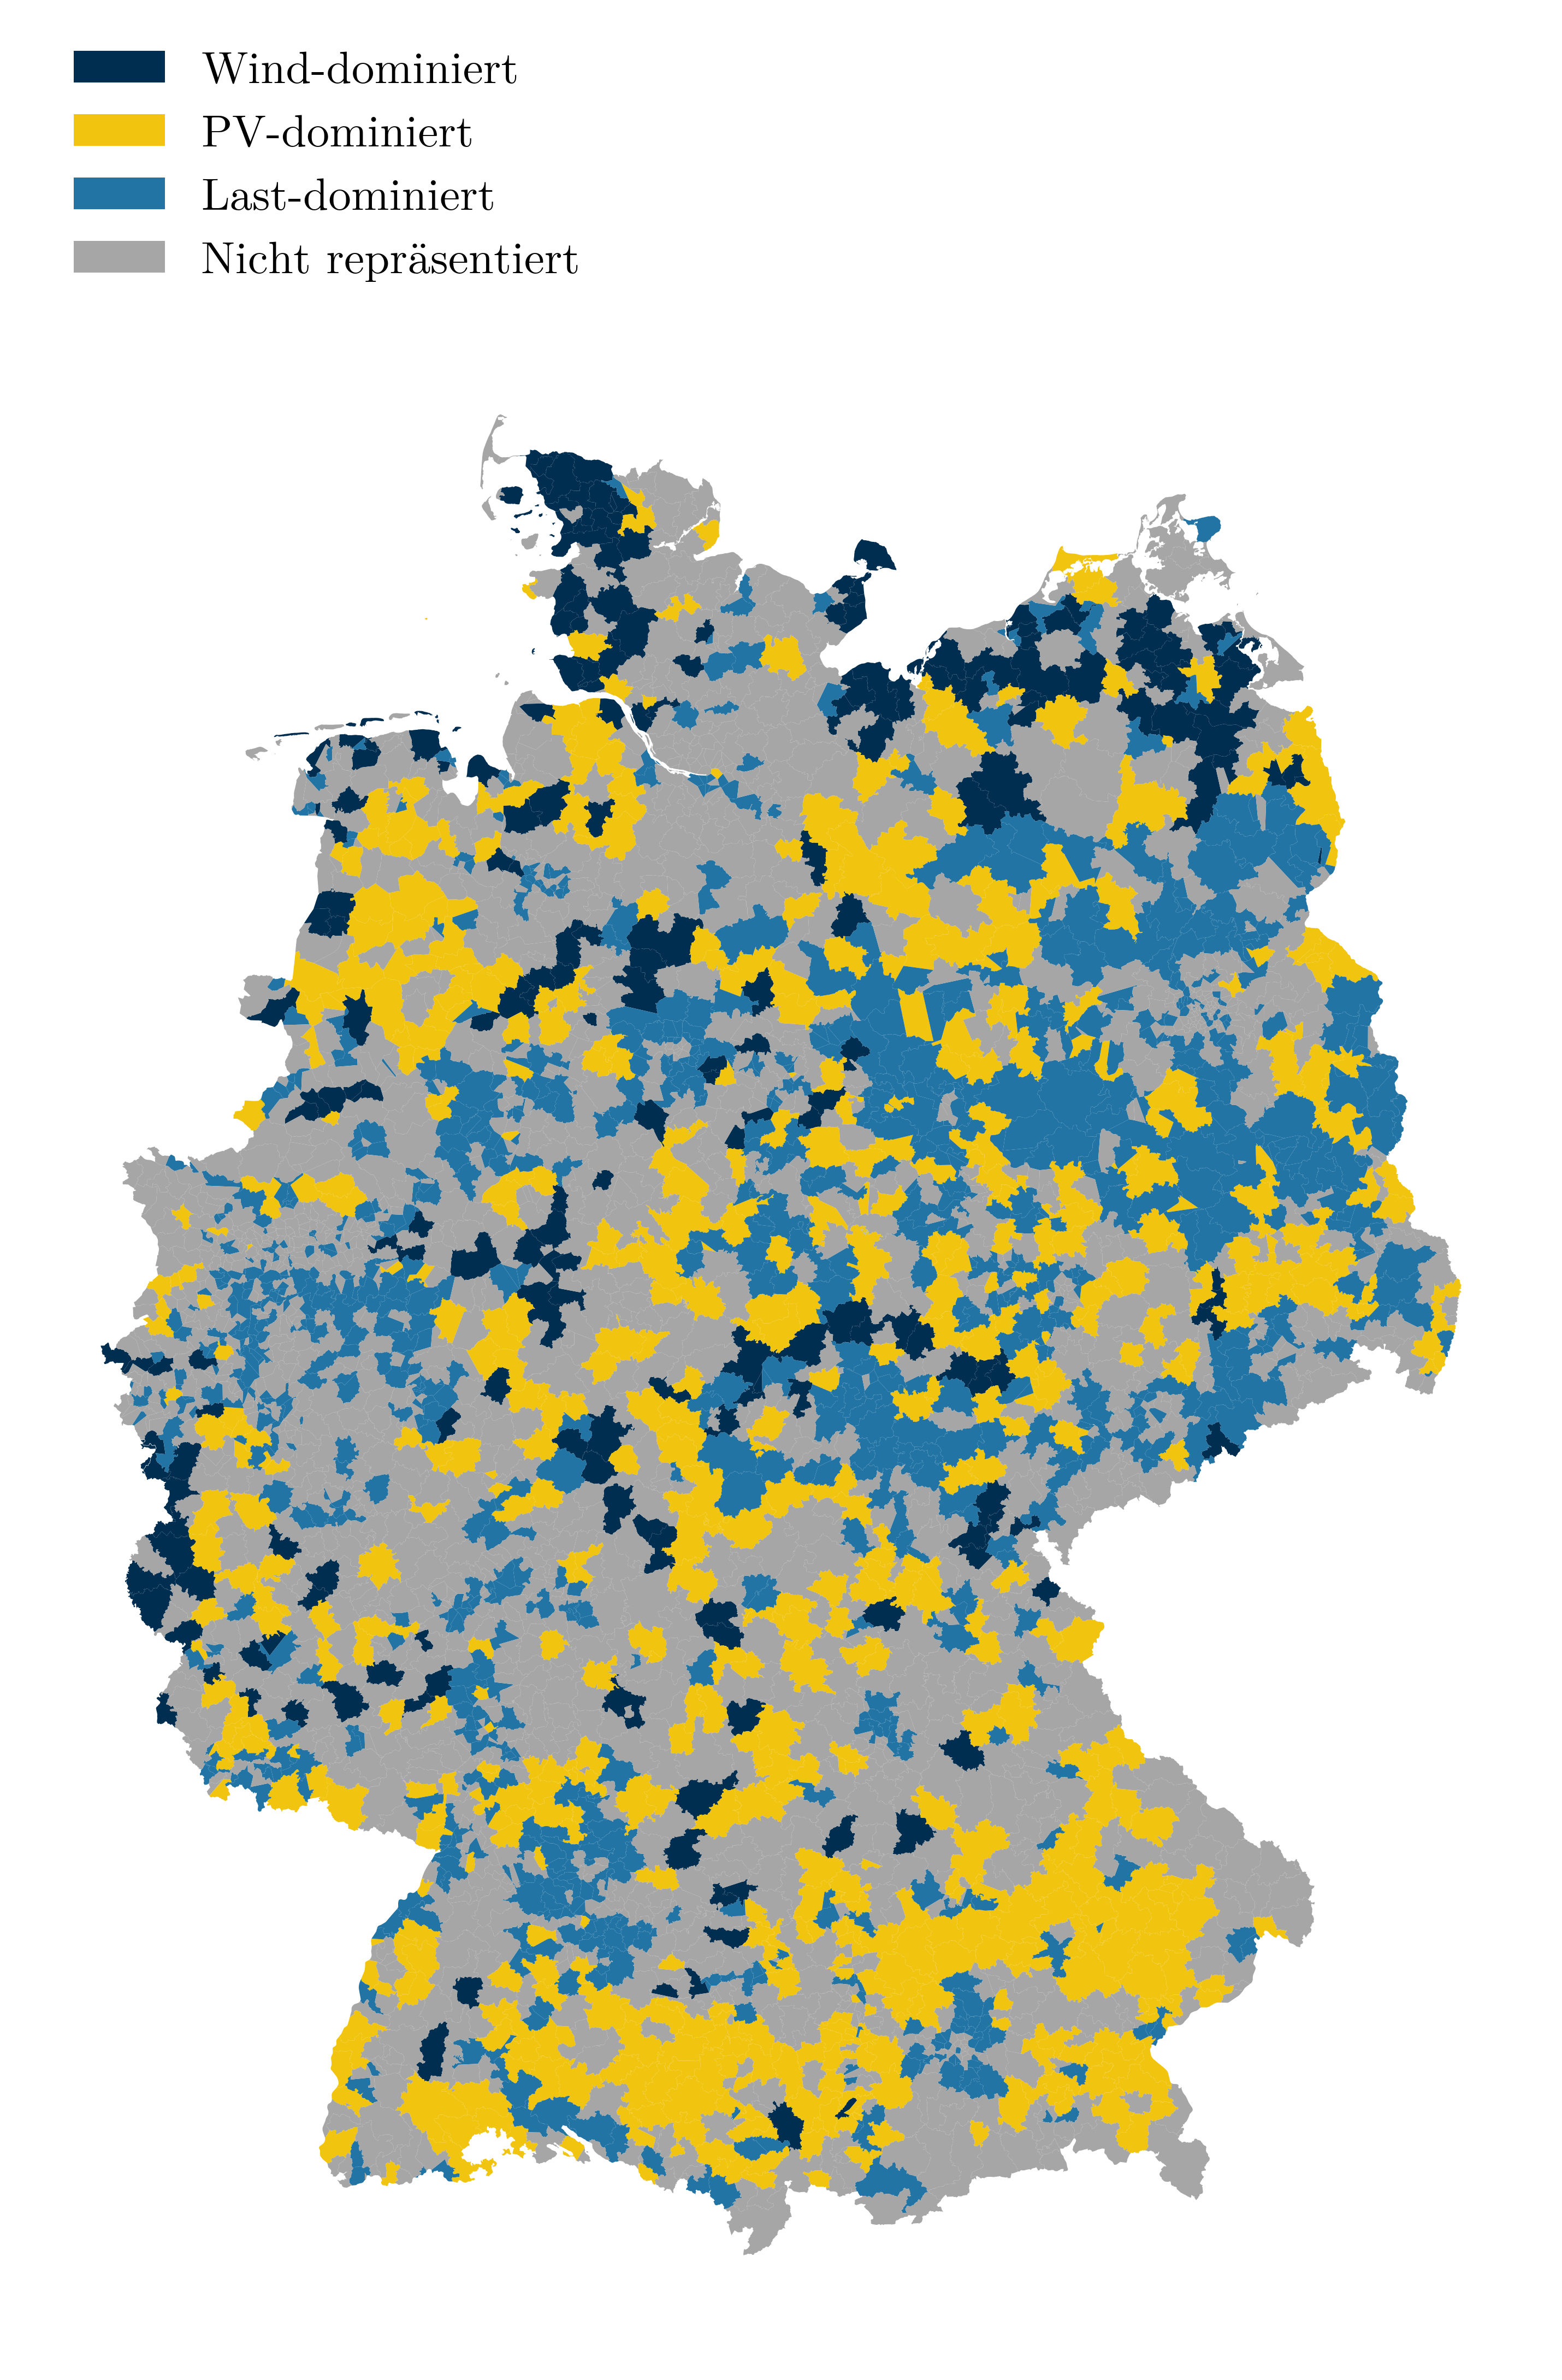
\includegraphics[width=\textwidth]{Bilder/clusters_representatives}
    \caption{Repräsentierte Netzgebiete in Deutschland}\label{fig:map_representatives}
\end{figure}


% TODO: Fahrzeuge je Netzgebiet und Szenario

\subsection{Charakteristik der Fahrtprofile}

% TODO: Fahrtstrecke berechnen mean +- Standardabweichung (je Regiotype?)
% TODO: Standzeit je Wegezweck mean +- Standardabweichung


Mit Hilfe des Software Tools \simbev (s. \autoref{chap:simbev_theo}) wurden für die zuvor geclusterten Referenznetzgebiet die Fahrtprofile der im Netzgebiet befindlichen Fahrzeuge erzeugt.
Die Charakteristik der Fahrtprofile spielt eine entscheidende Rolle für die Wirksamkeit der unterschiedlichen Ladestrategien und die Auswirkungen auf die Netze.
Hierbei steht vor allem der Anteil flexibilisierbarer und nicht-flexibilisierer Ladevorgänge, sowie die Gleichzeitigkeit von Ladevorgängen im Vordergrund.\medskip

Der Anteil flexibilisierbarer Ladevorgänge entspricht dem Anteil am Gesamtenergiebedarf, der an privaten Ladepunkten zu Hause oder am Arbeitsplatz nachgeladen wird.
Hierzu zählen alle Ladevorgänge die am Eigenheim, einer Wohnaalage oder auf einem Firmenparkplatz stattfinden.
Demgegenüber stehen nicht-flexibilisierer Ladevorgänge im öffentlichen Raum und an Schnellladestationen.
Je nach Raumtypen unterscheidet sich das Verhältnis leicht.
Im Mittel liegt der Anteil flexibilisierer Ladevorgänge über alle Szenarien innerhalb der einzelnen Gemeinden bei \SI{75.2}{\percent}.
Hiervon ausgenommen ist die \SzeFirmenparkplatzdot, bei der es aufgrund des geringeren Bestands an Ladeinfrastruktur am Arbeitsplatz zu mehr Ladevorgängen im öffentlichen Raum kommt.
Der Anteil nicht-flexibilisierer Ladevorgänge liegt bei dieser Szenarette bei \SI{70.0}{\percent}.
In \autoref{tab:ChargingShare} findet sich die entsprechende Aufteilung.

{
\renewcommand{\arraystretch}{1.2}% grßerer Zeilenabstand
\sisetup{range-phrase=~{--}~}% Gedankenstrich statt "bis" bei SIrange
\begin{table}[H]
	\begin{center}
		\caption{Aufteilung in flexibiliserbare und nicht-flexibiliserbare Ladevorgänge}
		\begin{tabu} to \textwidth {X[1] X[1, r] X[1, r]}
			\hline
								  					& \SzeFirmenparkplatzdot                               & Sonstige Szenarien                                   \\ \hline
			Flexibiliserbar$^{\mathrm{a}}$       	& \SI[separate-uncertainty = true]{70.0(24)}{\percent} & \SI[separate-uncertainty = true]{75.2(14)}{\percent} \\
			Nicht-flexibiliserbar$^{\mathrm{a}}$ 	& \SI[separate-uncertainty = true]{30.0(24)}{\percent} & \SI[separate-uncertainty = true]{24.8(14)}{\percent} \\ \hline
			\multicolumn{3}{l}{$^{\mathrm{a}}$Angabe als Anteil vom Gesamtenergiebedarf der Fahrzeuge mit Standardabweichung}
		\end{tabu}
		\label{tab:ChargingShare}
	\end{center}
	\vspace{-3mm}%Put here to reduce too much white space after your table
\end{table}
}

In \autoref{fig:example_load_profile} findet sich stellvertretend das \glspl{EPKW}-Lastprofil für ungesteuertes Laden einer mittelstädtischen Gemeinde (Raumtyp Nummer \num{73}) mit \num{6443} \glspl{EPKW} über eine Woche im Elektrifizierungs-Szenario (links).
Zusätzlich wurde die \SzeFirmenparkplatz (rechts) dargestellt.

\begin{figure}[H]
    \centering
    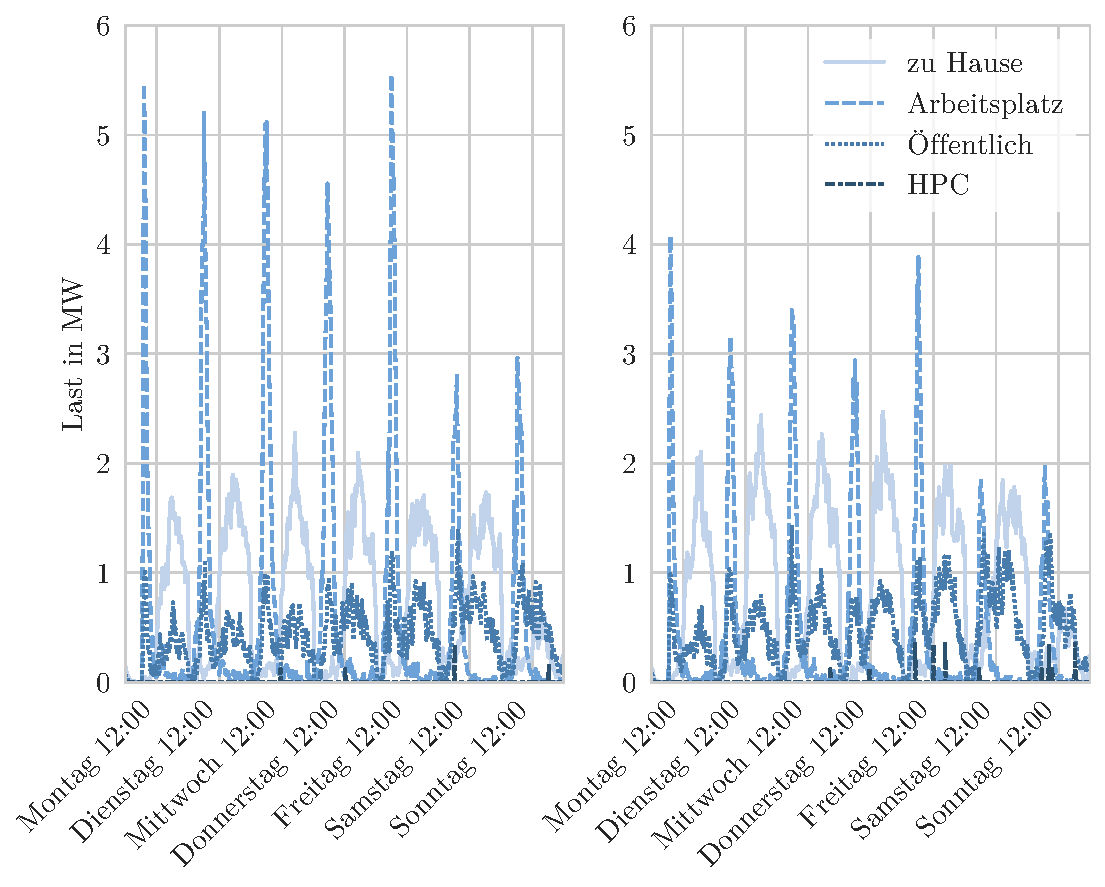
\includegraphics[width=\textwidth]{Bilder/example_load_profile}
    \caption{E-Pkw-Lastprofil für ungesteuertes Laden einer mittelstädtischen Gemeinde mit \num{6443} E-Pkws über eine Woche im Elektrifizierungs-Szenario (links) und der \SzeFirmenparkplatz (rechts)}\label{fig:example_load_profile}
\end{figure}

Die Lastgänge \zH und \Firmeparkplatz entsprechen den flexibilisierbaren Ladevorgängen im privaten Bereich. Unter dem Lastgang \oeffen sind hingegen alle öffentlichen Ladevorgänge mit Außnahme der Schnellladevorgänge (\gls{HPC}) zusammengefasst. Deutlich zu erkennen ist die hohe Gleichzeitigkeit am Vormittag sowohl am \Firmeparkplatz als auch im öffentlichen Raum, welche durch das Fahren zur Arbeit ausgelöst wird.
Auch die Rückkehr zum Wohnort ist ab dem frühen Nachmittag in den Lastgängen \zH und im öffentlichen Raum deutlich zu erkennen. Die entsprechenden Dauerlastkurven für die Gemeinde über die gleiche Woche (s. \autoref{fig:example_load_curve}) zeigen dies nochmals deutlich.
Schnellladevorgänge werden hingegen vermehrt am Wochenende ausgelöst, da verstärkt längere Fahrten angetreten werden.
Am Wochenende kommt es zusätzlich zu deutlich geringeren Anteilen von Ladevorgängen \zH und am \Firmeparkplatzdot, wodurch das Flexibilisierungspotential am Wochenende geringer ausfällt.
Gegenüber dem Elektrifizierungs-Szenario sinkt die Höchstlast in der \SzeFirmenparkplatzdot, jedoch sinkt auch das Flexibilisierungspotential bei gleichbleibendem Energiebedarf durch die Verschiebung der Ladevorgänge in den öffentlichen Raum.

\begin{figure}[H]
    \centering
    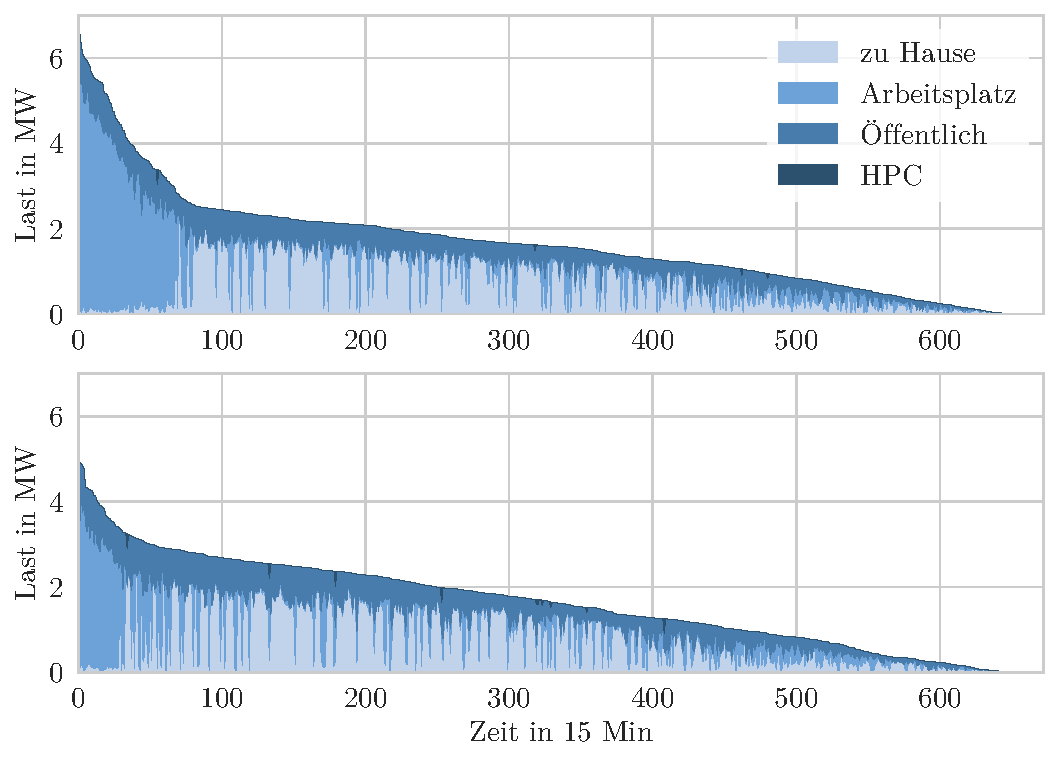
\includegraphics[width=\textwidth]{Bilder/example_load_duration_curve}
    \caption{E-Pkw-Dauerlastkurve für ungesteuertes Laden einer mittelstädtischen Gemeinde mit \num{6443} E-Pkws über eine Woche im Elektrifizierungs-Szenario (oben) und der \SzeFirmenparkplatz (unten)}\label{fig:example_load_curve}
\end{figure}


\subsubsection{Kritik}

Die erstellten Fahrtprofile spiegeln ein aus heutiger Sicht plausibel erscheinendes Bild wider.
Dennoch existieren einzelne Kritikpunkte, die innerhalb des \simbev Projektes gelöst werden sollten.
So war es zum Zeitpunkt der Erstellung der Fahrtprofile noch nicht möglich, einen längeren Zeitraum als eine Woche am Stück zu simulieren.
Da sich jedoch die Netzuntersuchungen im Rahmen dieser Masterarbeit auf einen Zeitraum von einem Jahr beziehen, wird die simulierte Woche stellvertretend für das gesamte Jahr verwendet.
Hierfür wurde jedes Fahrtprofil solange mit sich selbst verlängert und logisch verknüpft, bis die gewünschte Länge erreicht wurde.
Dieses bringt jedoch einige Nachteile mit sich.
Durch den kurzen simulierten Zeitraum fällt der \gls{SOC} einiger Fahrzeuge im Laufe der Woche nur geringfügig.
Es ist zu vermuten, dass dies dazu führt, dass Ladevorgänge an Schnellladeinfrastruktur un­ter­re­prä­sen­tiert dargestellt werden.
Auch nimmt der Ladebedarf im öffentlichen Raum im Laufe der Woche zu.
Dies lässt sich durch die Abhängigkeit der Ladewahrscheinlichkeit vom \gls{SOC} erklären, da der \gls{SOC} im Mittel im Verlaufe des Woche sinkt.


\subsection{Ergebnisse der Implementierung der Ladestrategien}\label{chap:results_charging_strategies}


\subsection{Verteilung der Last auf die Ladeinfrastruktur}\label{chap:distribute_demand_ev}

% TODO: Schnittmenge Gemeinden <-> Netzgebiet erklären -> Karte!
% TODO: Grafik elia Bericht


\subsection{Abregelungsbedarf innerhalb der untersuchten Netzgebiete}

